\documentclass[
	english,
	fontsize=10pt,
	parskip=half,
	titlepage=true,
	DIV=12
]{scrartcl}

\usepackage[utf8]{inputenc}
\usepackage{babel}
\usepackage[T1]	{fontenc}
\usepackage{lmodern}
\usepackage{microtype}
\usepackage{color}
\usepackage{csquotes}
\usepackage{tabto}

\usepackage{hyperref}

\usepackage{graphicx}
\usepackage{wrapfig}
\usepackage[bf]{caption}
	\captionsetup{format=plain}

\newcommand*{\tabcrlf}{\\ \hline}

\usepackage{amsmath}

\usepackage{minted}
	\usemintedstyle{friendly}

\newcommand*{\inPy}[1]{\mintinline{python3}{#1}}
\newcommand*{\ie}{i.\;e. }
\newcommand*{\eg}{e.\;g. }

\newcommand{\thus}{\ensuremath{\rightarrow}}

\begin{document}

\part*{Python Problems 03, Spring 2021}
\section{Cross Sum (1 P)}
Write a function that takes an integer for an argument and returns the cross sum of this number.

\section{Erroneous Code (1 P)}
Explain, why the below code does \emph{not} work, \ie why in the output, \texttt{x} and \texttt{y} are not swapped.
\begin{minted}[linenos]{python}
def swap(x, y): 
    temp = x
    x = y
    y = temp
  
# Driver code 
x = 2
y = 3
swap(x, y) 
print(x) 
print(y) 
\end{minted}


\section{FizzBuzz (1 P)}
In the Game \emph{FizzBuzz}, players count from one upwards. If a number is divisible by three, the player should not name the number, but say \emph{Fizz}. If the number is divisible by five, players should say \emph{Buzz}. If the number is both, divisible by three and five, players say \emph{Fizzbuzz}. Hence, players count like this:
\begin{center}
	1, 2, Fizz, 4, Buzz, Fizz, 7, 8, Fizz, Buzz, 11, Fizz, 13, 14, FizzBuzz ...
\end{center}

Create a program that puts this sequence on the screen.

\emph{Optionally: (+1 P)}\\
Write your code such that it can be expanded easily. Instead of placing the output directly on screen, put the numbers/\emph{Fizz}es and \emph{Buzz}es into a data container. Make it such that you can easily change the divisors and the replacement words. Can you find a structure that allows for defining an arbitrary count of divisor-substitution pairs? It \emph{is} possible to write a program, that, by adding only a single extra line, allows to expand the rules to say \emph{Tess} if a number is divisible by 7.

\section{Random/Drunk Walk (1 P)}
Imagine a drunkard, stumbling down a road. With each step forward, the drunkard will stagger randomly to the left or right.

Write a program that simulates how far the drunkard has veered off to the left or right after $N$ steps forward. For the basic version of this problem, we'll assume that the drunkard is stumbling along a road of \emph{infinite width}, \ie going to either direction is always possible.

\emph{Optional (+1 P)}:\\
Assume now, the drunkard is a bit lopsided: the probability of going left/right is no longer 50/50, but \eg 40/60 or any other distribution. Expand your code to include this bias.

\emph{Optional (+1 P)}:\\
Drop the assumption that the road has infinite width; instead, include a width $W$ in your model. Your drunkard starts in the middle of the road. If they have veered off $^{W}/_{2}$ steps in either direction, they cannot go any further into that direction; instead, they either rebound at the walls (\ie \eg go left instead of right), or graze the wall (\ie go in a straight line). It is your choice which of the two you implement; if you want to, do both and make it a random decision if the drunkard rebounds or goes on straight.

\emph{Optional (+1 P)}:\\
Make your code run multiple times with a fixed number of steps $N$, and store the result of each run. Create a \emph{histogram} from this list of outcomes, \ie a listing of \emph{how often} each individual outcome occured after sending $K$ drunkards down your street of length $N$ (and possibly width $W$). Plot your results in a (text based) bar chart. Your output could look like this:
\begin{minted}{text}
Drift
-5 #
-4 ###
-3 ##
-2 #######
-1 ##########
 0 ################
 1 #####
 2 ########
 3 ###
 4 #
 5
\end{minted}

\emph{Background Information:}\\
The model of a \emph{random walk} or \emph{drunk walk} is often the basis for statistical analysis of scenarios where one of several outcomes is bound to occur. Fields where this can be used cover polymer chemistry, magnetism, lifetime of electronic parts, ... -- you name it. You can derive tons of useful information from implementing this very basic concept.

\section{$\pi$ from the Monte Carlo Method (1 P)}
\begin{wrapfigure}{r}{.25\linewidth}
\vspace{-20pt}
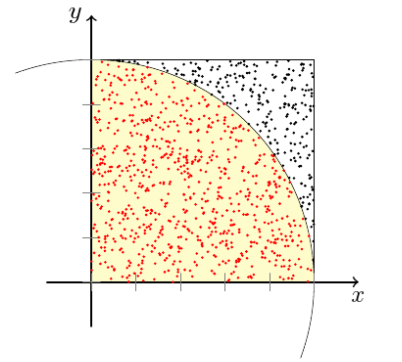
\includegraphics[width=\linewidth]{MCarlo}
\caption{\url{https://commons.wikimedia.org/wiki/File:Pi_statistisch.png}}
\label{fig:MCPI}
\vspace{-50pt}
\end{wrapfigure}
%
Write a function that approximates the value of $\pi$. To do so, follow these instructions:
\begin{itemize}
\item Generate $N$ pairs of positive random numbers $x, y$ between 0 and 1.
\item For each pair of numbers, compute $x^2 + y^2$
\item For each pair $(x, y)$ where this expression is less than or equal to one, increase a counter.
\item For big $N$, the expression $\frac{\text{counter}}{N}$ approaches $\frac{\pi}{4}$
\end{itemize}

Write your function such that you can pass $N$ as an argument. This parameter controlls the accuracy of your approximation of $\pi$.

\emph{Note}: You'll need very big values of $N$ to get half-decent results. If your algorithm outputs something like $3.13$, you've probably done everything correctly.

\emph{Background Information}:\\
Using Pythagoras' theorem, we find that the distance between the origin $(0, 0)$ and some point $(x, y)$ can be computed from
\[ R^2 = x^2 + y^2 \]
If we now fix some value for $R$, we can compute for any point $(x, y)$ whether it is within or outside of a circle of radius $R$. For simplicity, we choose $R = 1$. Since $1^2 = 1$, we find that the algorithm described above counts how many points are within a circle of radius 1.

We are randomly picking points $(x, y)$ from the interval $[0, 1] \times [0, 1]$, \ie a square of unit length, coinciding with the first quadrant of the unit circle centered in origin (cf. figure \ref{fig:MCPI}). Counting the number of dots within the circle amounts to measuring the \emph{area of a quadrant of the circle} in units of the \emph{area of the square}.

As you know, for the area of the circle, it holds:
\[ A = R^2 \cdot \pi \]

Plugging in $R^2 = 1$ and acounting for the factor 4 (we're only covering a quadrant of the circle) gives the above algorithm.

\emph{Background Information}:\\
Monte Carlo Methods are a collection of techniques often used where accuracy has to be sacrificed for computation time. Albeit not terribly precise, they often are the only means of evaluating some integrals. We'll do a mini excursion on them at the end of our course.


\section{Prime Number Sieve (2 P)}
Computing quotients (and hence also the remainder of a division, \ie the modulus) is a relatively costly operation: it takes about ten times longer than an addition (on usual processor architectures). We want to avoid divisions when solving time critical problems.

The \emph{Sieve of Eratosthenes} (named after Eratosthenes of Kyrene, born in ancient Greece, between 276 and 273 BCE) is an algorithm for finding all prime numbers between 2 and some arbitrary upper boundary $N$ that works \emph{without division/modulus}.

Implement Eratosthenes sieve. To do so, create a list of length $N+1$ and fill it with all integers between $0$ and $N$. Then, eliminate all multiples of 2 from your list (\eg by setting them to 0). Continue by eliminating all multiples of 3, and so on, unless the number in question has already been eliminated. For example, you need not eliminate all multiples of four, since four has been removed when eliminating all multiples of 2. Skip the fours and go on to the fives, and so on.

\section{Text To List (1 P)}
Write a program that takes a string of numbers separated by commas and that computes a \inPy{list} containing the numbers from this.

\emph{Example}:\\
Input: \texttt{"1, 5, 99, -3, 5.7"} \tab
Output: \texttt{[1, 5, 99, -3, 5.7]}

\emph{Hint:} This can be done with a single line of code.
\end{document}
